
%NO PREAMBLE, NO \begin{document} or \usepackage here !

\subsection{Вопрос 3. Эффект Яна-Теллера}

\subsection*{определение}
Любая нелинейная молекула в вырожденном электронном состоянии будет искажаться и понижать свою симметрию, тем самым приводя к снятию вырождения.

Z-лиганды могут удаляться или приближаться к центральному атому, уменьшая взаимодействие L с орбиталями $d_z^2$, $d_{xz}$, $d_{yz}$.

Ниже показаны эффекты Я.-Т. для каждого из вариантов заполнения $d$ орбитали.

\begin{figure}[H]
\centering
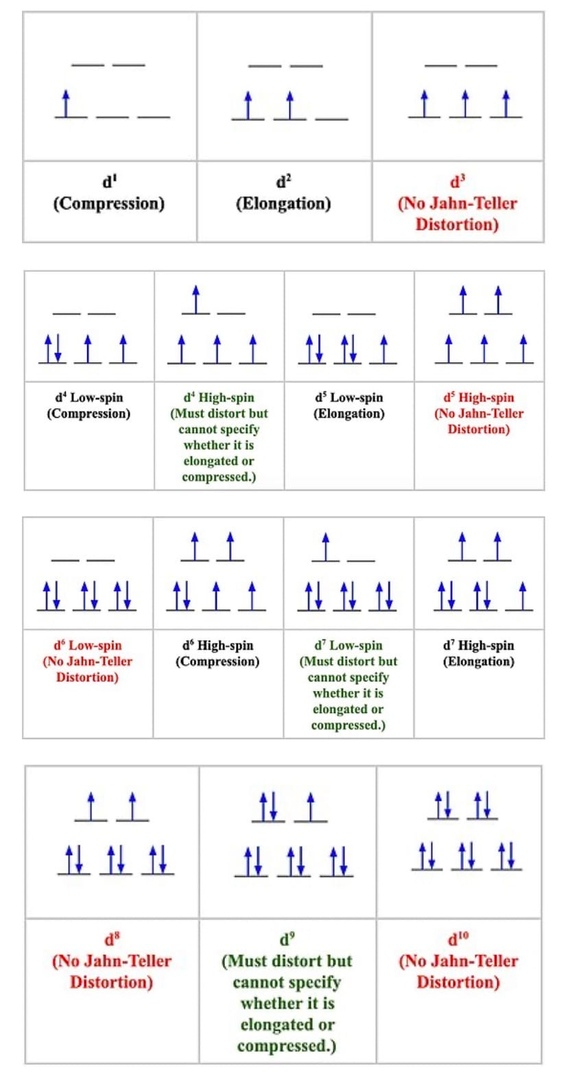
\includegraphics[scale=.500]{/home/someanonimcoder/TeX/tic_summer/images/yan-teller.jpg}
\end{figure}

\subsection*{Статический и динамический эффекты}

Динамический эффект Я.-Т. -- переходы между жвумя минимумами. Требует низкого барьера между минимумами.

Статический эффект Я.-Т. -- большой барьер между минимумами, стабильное нахождение в одном из минимумов.

